\documentclass[12pt]{article}
\oddsidemargin=0.0in
\evensidemargin=0.0in
\textwidth=6.5in
\topmargin=-0.55in
\textheight=9.3in
\usepackage{hyperref}
\usepackage{graphicx}
\usepackage{amsmath}

\begin{document}
\pagestyle{empty}
 
\begin{center}
{\LARGE {\bf Homework Seven}}\\
\bigskip
{\Large {\bf Calculus I}}\\
\bigskip
{\Large {\bf College of the Atlantic}}\\
\bigskip
{ {\bf Due Friday, October 28, 2022}}\\ 
\end{center}
\medskip

\noindent There are two parts to this assignment.\\

\noindent {\bf Part 1: WeBWorK}.  Do Homework 07A and 07B on
WeBWorK.  The WeBWorK page is here: 
\url{https://webwork.runestone.academy/webwork2/coa-feldman-es1024i-fall-2022/}.
I recommend doing the WeBWorK part of the homework first.  This will
enable you to benefit WeBWorK's instant feedback before you do part
two.\\ 


\noindent {\bf Part 2: Non-WeBWorK problems}.  Here are some
instructions for how to submit this part of the assignment.
\begin{itemize}
  \setlength{\itemsep}{0mm}
\item Do the problems by hand using pencil (or pen) and paper.
  There is no need to type this assignment.
%\item If you like working on a tablet, go for it. 
\item Make a pdf scan of your work using genius scan or some
  similar scanning app.  Please make the homework into a single
  pdf, not multiple pdfs.
\item Submit the assignment on google classroom.  Please don't
  email it to me.
  %(Between my two classes I will be receiving
  %around 60 assignments a week.  Keeping track of them all in email 
  %is challenging.)
\item If you want, you can do the non-WeBWorK problems in pairs and
  submit only one assignment for the two of you. \\
\end{itemize}

\noindent Here are some non-WeBWorK problems.\\


\begin{enumerate}
\setlength{\itemsep}{33mm}

\item 
  \begin{enumerate}
    \setlength{\itemsep}{8mm}
  \item Find the equation of the line tangent to $f(x) = \ln(x)$ at
    $x=1$.
  \item What is the value of the tangent line at $x=1.01$, $x=1.1$,
    and $x=2$?
  \item What are the values of $\ln(x)$ at $x=1.01$, $x=1.1$,
    and $x=2$?
  \item Are the values of the tangent line above or below $\ln(x)$?
    How is your answer related to the concavity of $\ln(x)$? A sketch
    of the function and the tangent line will be helpful. 
  \end{enumerate}

\newpage
  
\item Consider the scenario illustrated in the figure: a metal bar of
  length $\ell$ is attached to a point P on the edge of a circle of
  radius $a$. The point Q, at the other end of the metal rod, slides
  back and forth along the $x$ axis.  Note that the triangle OPQ is
  \emph{not} a right triangle.
  \begin{enumerate}
    \setlength{\itemsep}{10mm}
  \item Find an expression for $x$ as a function of the angle
    $\theta$. Your answer will have an $a$ and and $\ell$ in it.
  \item $x(\theta)$ for the values $a=3$ and $\ell = 8$. Does the
    plot make sense?
    \item Suppose the circle is rotating at a rate of $2$ radians per
      second, and that $a = 3$ cm and $\ell = 8$ cm.
      \begin{enumerate}
        \setlength{\itemsep}{5mm}
      \item How fast is the point Q moving when $\theta = \pi/4$?
      \item How fast is the point Q moving when $\theta = \pi/2$?
      \item How fast is the point Q moving when $\theta = \pi$?
      \item How fast is the point Q moving when $\theta = 3\pi/2$?
      \end{enumerate}
     \item Do the signs and magnitudes of the speeds you found above
       make sense? Explain briefly. 
  \end{enumerate}

  \phantom{blah}

  \phantom{blah}
  
  \phantom{blah}


\begin{figure}[h]
\begin{center}
\vspace{1mm}
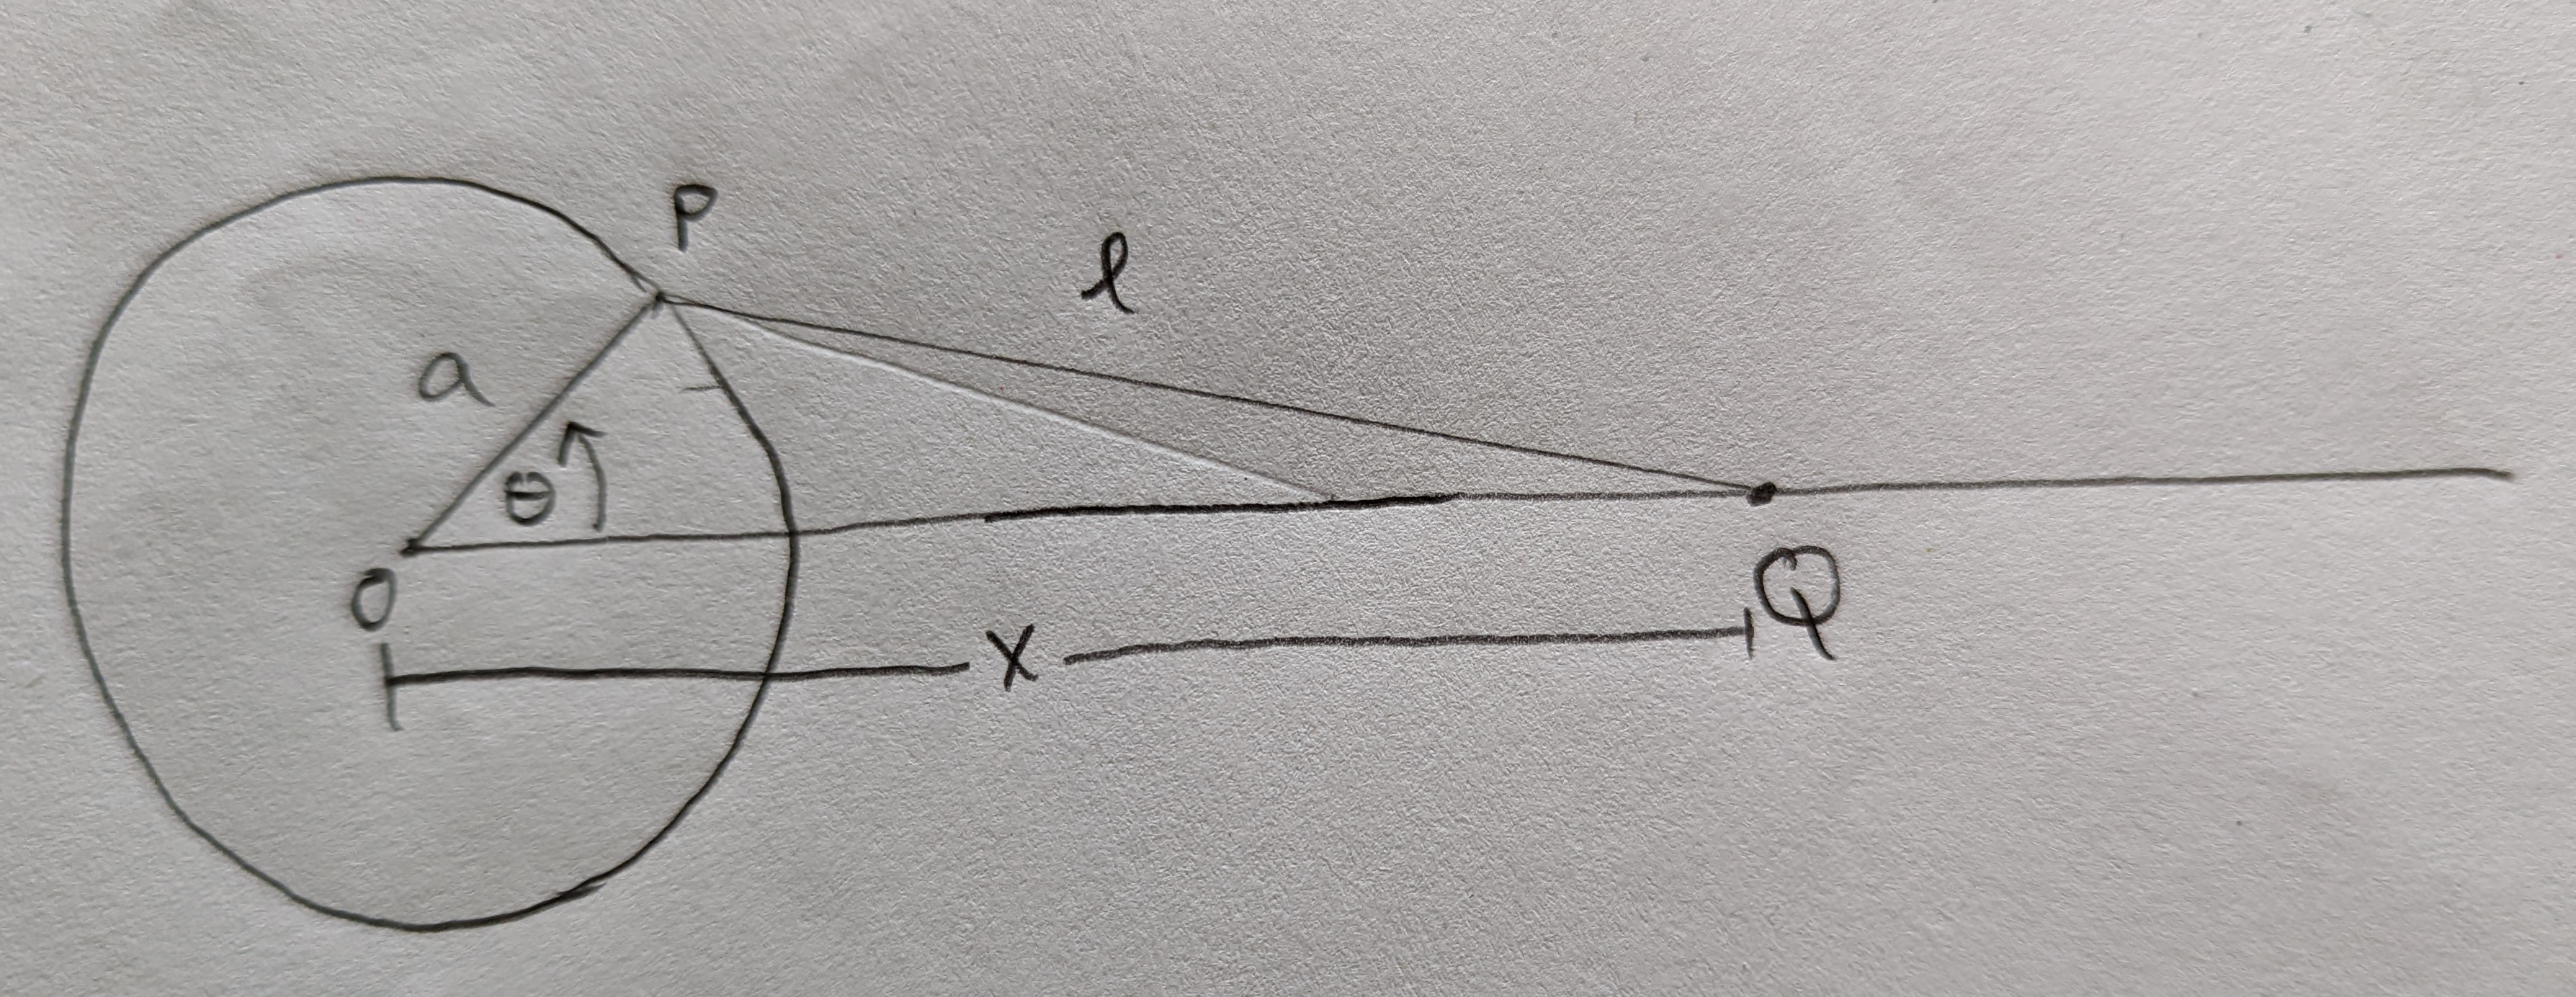
\includegraphics[width=7.0in]{hw07_figure.png}
\vspace{-2mm}
%\caption{The position of a object (in meters) as a function of time
%  (in seconds). }
%\label{fig:graph2}
\vspace{-5mm}
\end{center}
\end{figure}
  
  
\end{enumerate}

\end{document}




  \item Determine an equation for the linear function that generates
    the values in the table below.  

\begin{center}
\begin{tabular}{|| l | l ||}
\hline $x$ & $f(x)$ \\
\hline
5.2 & 27.8 \\
5.3 & 29.2 \\
5.4 & 30.6 \\
5.5 & 32.0 \\
5.6 & 33.4 \\
\hline
\end{tabular}
\end{center}





\end{document}
